\documentclass{article}
\usepackage[pdftex]{graphicx,color}
\usepackage{amsmath}
\usepackage{url}

\newcommand{\dealii}{{\textsc{deal.II}}}
\newcommand{\pfrst}{{\normalfont\textsc{p4est}}}
\newcommand{\trilinos}{{\textsc{Trilinos}}}
\newcommand{\aspect}{\textsc{Aspect}}

\begin{document}

\thispagestyle{empty}
\vspace*{.3\textheight}

\begin{centering}
  \parindent0pt
  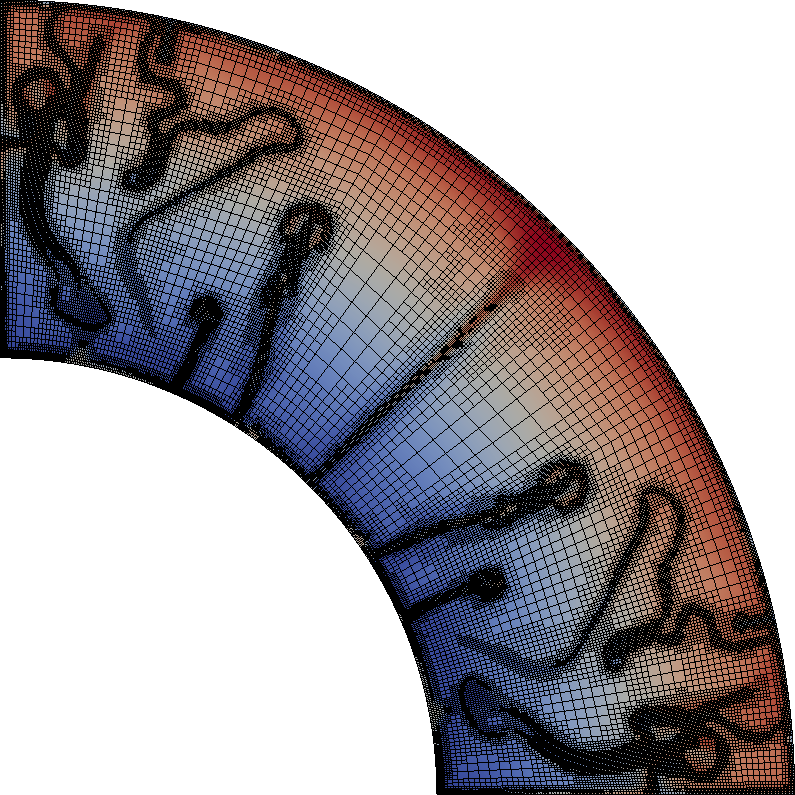
\includegraphics[width=0.6\textwidth]{mesh-2d.png}

  \vfill

  {\Large \aspect{} 0.8 preview release}
  \\[1cm]
  {\large
    Wolfgang Bangerth\\
    Timo Heister\\
    Martin Kronbichler\\
  }
\end{centering}


\pagebreak

\tableofcontents

\pagebreak

\section{Introduction}

\section{Equations, models, coefficients}

\subsection{Basic equations}

\aspect{} solves the following system of equations in a two- or
three-dimensional domain $\Omega$:
\begin{align}
  \label{eq:stokes-1}
  -\nabla \cdot 2\eta \varepsilon(\mathbf u) + \nabla p &=
  \rho \mathbf g
  & \qquad
  & \textrm{in $\Omega$},
  \\
  \label{eq:stokes-2}
  \nabla \cdot (\rho \mathbf u) &= 0
  & \qquad
  & \textrm{in $\Omega$},
  \\
  \label{eq:temperature}
  \rho c_P \left(\frac{\partial T}{\partial t} + \mathbf u\cdot\nabla T\right)
  - \nabla\cdot k\nabla T
  &=
  \gamma ...
  & \qquad
  & \textrm{in $\Omega$},
\end{align}
where $\varepsilon(\mathbf u) = \frac{1}{2}(\nabla \mathbf u + \nabla\mathbf
u^T)$ is the symmetric gradient of the velocity (often called the
\textit{strain rate}).

In this set of equations, \eqref{eq:stokes-1} and \eqref{eq:stokes-2}
represent the compressible Stokes equations in which $\mathbf u=\mathbf
u(\mathbf x,t)$ is the velocity field and $p=p(\mathbf x,t)$ the pressure
field. Both fields depend on space $\mathbf x$ and time $t$. Fluid flow is
driven by the gravity force that acts on the fluid and that is proportional to
both the density of the fluid and the strength of the gravitational pull.

Coupled to this Stokes system is equation \eqref{eq:temperature} for the
temperature field $T=T(\mathbf x,t)$ that contains heat conduction terms as
well as advection with the flow velocity $\mathbf u$.
.......talk about rhs

These equations are
augmented by boundary conditions that can either be of Dirichlet-, Neumann, or
tangential type on subsets of the boundary $\Gamma=\partial\Omega$:
\begin{align}
  \mathbf u &= 0 & \qquad &\textrm{on $\Gamma_{0,\mathbf u}$},
  \\
  \mathbf n \cdot \mathbf u &= 0 & \qquad &\textrm{on $\Gamma_{\parallel,\mathbf u}$},
  \\
  T &= T_{\text{prescribed}}
   & \qquad &\textrm{on $\Gamma_{D,T}$},
  \\
  \mathbf n \cdot k\nabla T &= 0
   & \qquad &\textrm{on $\Gamma_{N,T}$}.
\end{align}
Here,
$\Gamma_{0,\mathbf u}$ corresponds to parts of the boundary on which the
velocity is fixed to be zero,
$\Gamma_{\parallel,\mathbf u}$ to parts of the boundary on which the
velocity may be nonzero but must be parallel to the boundary,
where
$\Gamma_{D,T}$ to places where the temperature is prescribed (for example at
the inner and outer boundaries of the earth mantle), and finally
$\Gamma_{N,T}$ to places where the temperature is unknown but the heat flux
across the boundary is zero (for example on symmetry surfaces if only a part
of the shell that constitutes the domain the Earth mantle occupies is
simulated). We require that one of these boundary conditions hold at each
point for both velocity and temperature, i.e.,
$\Gamma_{0,\mathbf u}\cup\Gamma_{\parallel,\mathbf u}=\Gamma$ and
$\Gamma_{D,T}\cup\Gamma_{N,T}=\Gamma$.

\aspect{} solves these equations in essentially the form stated. In
particular, the form given in \eqref{eq:stokes-1} implies that the pressure
$p$ we compute is in fact the \textit{total pressure}, i.e., the sum of
hydrostatic pressure and dynamic pressure.%
\footnote{Other codes often replace this equation by $-\nabla \cdot 2\eta
  \nabla \mathbf u + \nabla p_d =
  (\rho-\rho_0) \mathbf g$ where $p_d=(p+\rho_0 \varphi)$, and $\phi$ is the
  gravitational potential so that
  $\mathbf g=-\nabla\varphi$ and chosen in such a way that $\varphi=0$ at that
  part of the boundary where we want the pressure to be zero (e.g., on the
  earth surface). Furthermore, $\rho_0$ is a reference density. In this
  formulation, it is clear that the quantity that drives the fluid flow is in
  fact the \textit{buoyancy} caused by the \textit{variation} of densities,
  not the density itself. $p_d=p+\rho_0 \varphi$ is then the \textit{dynamic}
  pressure, i.e., the difference between total pressure and hydrostatic
  pressure $p_s=-\rho_0\varphi$.

  While this formulation has a number of numerical advantages, it also has
  significant disadvantages: (i) The pressure we compute is not immediately
  comparable to quantities that we need to look up pressure-dependent
  quantities such as the density. (ii) The definition of a reference density
  is only simple if we have incompressible models for which the density only
  depends on the temperature; for more complicated models, it is not a priori
  clear which density $\rho_0$ to chose so that $p+\rho_0 \varphi$ really only
  contains the dynamic part of the pressure. (iii) To compute the total
  pressure $p$ from $p_d$ one needs to know a gravitational potential
  $\varphi$ that is consistent with the gravity vector $\mathbf g$. This is
  not always trivial because many simple models just prescribe a $\mathbf g$
  for which no such potential needs to exist; for example, this is the case
  when using a radially inward gravitational vector of constant magnitude.}
Consequently, it allows the direct use of this pressure when looking up
pressure dependent material parameters.

In the implementation of these equataions, \aspect{} uses the SI unit system
throughout (i.e., it expresses all quantities in meters, kilograms and
seconds). All material parameters, geometries, etc., must also be expressed in
these units. For convenience, some rate-type output quantities are provided in
units \textit{per year} instead of \textit{per second}; however, this
conversion happens at the time output is generated, and is not part of the
solution process.


\subsection{Coefficients}

The equations above contain a significant number of coefficients that we will
discuss in the following. In the most general form, many of these coefficients
depend nonlinearly on the solution variables pressure $p$, temperature $T$
and, in the case of the viscosity, on the strain rate $\varepsilon(\mathbf
u)$. Alternatively, they may be parameterized as a function of the spatial
variable $\mathbf x$. \aspect{} allows both kinds of parameterizations.

\textbf{Note: The next version of \aspect{} will actually iterate out
  nonlinearities in the material description. However, in the current version,
  we simply evaluate all nonlinear dependence of coefficients at the solution
  variables from the previous time step or a solution suitably extrapolated from
  the previous time steps.}

Note that below we will discuss examples of the dependence of coefficients on
other quantities; which dependence is actually implemented in the code is a
different matter. As we will discuss in Section~\ref{sec:parameters} and
\ref{sec:extending}, some versions of these models are already implemented and
can be selected from the input parameter file; others are easy to add to
\aspect{} by providing self-contained descriptions of a set of coefficients
that the rest of the code can then use without a need for further
modifications.

Concretely, we consider the following coefficients and dependencies:
\begin{itemize}
\item \textit{The viscosity $\eta=\eta(p,T,\varepsilon(\mathbf u),\mathbf
    x)$:} Units $\textrm{Pa}\cdot \textrm{s} =
  \textrm{kg}\frac{1}{\textrm{m}\cdot\textrm{s}}$.

  The viscosity is the proportionality factor that relates total forces
  (external gravity minus pressure gradients) and fluid velocities $\mathbf
  u$. The simplest models assume that $\eta$ is constant, with the constant
  often chosen to be on the order of $10^{21} \textrm{Pa}\;\textrm{s}$.

  More complex (and more realistic) models assume that the viscosity depends
  on pressure, temperature and strain rate. Since this dependence is often
  difficult to quantify, one modeling approach is to make $\eta$ spatially
  dependent.

\item \textit{The density $\rho=\rho(p,T,\mathbf x)$:} Units
  $\frac{\textrm{kg}}{\textrm{m}^3}$.

  In general, the density depends on pressure and temperature, both through
  pressure compression, thermal expansion, and phase changes the material may
  undergo as it moves through the pressure-temperature phase diagram.

  The simplest parameterization for the density is to assume a linear
  dependence on temperature, yielding the form
  $\rho(T)=\rho_{\text{ref}}[1-\beta (T-T_{\text{ref}})]$ where
  $\rho_{\text{ref}}$ is the reference density at temperature $T_{\text{ref}}$
  and $\beta$ is the linear thermal expansion coefficient. For the earth
  mantle, typical values for this parameterization would be
  $\rho_{\text{ref}}=3300\frac{\textrm{kg}}{\textrm{m}^3}$,
  $T_{\text{ref}}=293 \textrm{K}$, $\beta=2\cdot 10^{-5}
  \frac{1}{\mathrm{K}}$.

\item \textit{The gravity vector $\mathbf g=\mathbf g(\mathbf x)$:} Units
  $\frac{\textrm{m}}{\textrm{s}^2}$.

  Simple models assume a radially inward gravity vector of constant magnitude
  (e.g., the surface gravity of Earth, $9.81 \frac{\textrm{m}}{\textrm{s}^2}$),
  or one that can be computed analytically assuming a homogenous mantle
  density.

  A physically self-consistent model would compute the gravity vector as
  $\mathbf g = -\nabla \varphi$ with a gravity potential $\varphi$ that
  satisfies $-\Delta\varphi=4\pi G\rho$ with the density $\rho$ from above and
  $G$ the universal constant of gravity. This would provide a gravity vector
  that changes as a function of time. Such a model is not currently
  implemented.

\item $c_P$
\item $k$
\item $\gamma$
\end{itemize}


\subsection{Numerical methods}

Provide outline, refer to papers

\subsection{Variations on the basic equations}

Boussinesq approximation. Incompressible Stokes.

\section{Installation}

\section{Running \aspect}

Output in MKS, occasionally per year

\section{Input parameters}
\label{sec:parameters}

\section{Extending \aspect}
\label{sec:extending}

deal.II
documentation
dimension independent

plugins
existing plugins have header files so they show up in the documentation but
     this is not necessary

\end{document}
